%*********************第二章******************
\chapter{使用``目标候选''提高跟踪器的尺度和宽高比适应力}
\label{chapbmvc}

\section{引言}
绪论已经介绍过,视觉跟踪器是视频监控、人机交互、智能导航等应用领域至关重要的基础。
从上世纪80年代的KLT跟踪器\upcite{lkoptflow, klt2},到最新提出的深度学习跟踪器\upcite{deepimage, deeptrack},
视觉跟踪已经被研究了几十年。
但随着应用需求的不断提升,应用场景的日趋复杂,很多问题仍然未得到有效解决。
跟踪器对目标物体的尺度和宽高比的适应力就是这些问题之一。

跟踪算法的基础研究一般面向最为通用的跟踪器类别,即``短时间、单目标、无模型''跟踪器。
``短时间''是一个相对概念,通常意指用于跟踪的是较短的视频序列(通常从几百帧到几千帧),而不是直接进行长时间的在线跟踪。
``单目标''即被跟踪的目标物体只有一个,跟踪过程中不考虑其它物体的位置和状态。
``无模型''指的是不依赖跟踪目标的任何先验信息,不在跟踪前对目标物体进行任何建模。
跟踪算法中最为通用的结果表示方式是``边界框'',即在图像帧中紧密包围目标物体的矩形框。
跟踪过程中,目标物体可能发生复杂的运动、旋转、形变等。
体现在结果上,就是边界框的位置、尺度和宽高比发生变化。
如果跟踪器边界框的尺度和宽高比无法随物体发生变化,那么跟踪结果仅能体现出物体的位置信息,而无法描述其它物体状态。
除此之外,不准确的边界框还将导致跟踪过程中不准确的目标/背景分割。
过多的非目标物体信息可能包含在边界框中,而部分目标物体信息却可能在边界框外。
这些误差将在物体描述中积累,积累到一定程度,跟踪器将出现偏移(Drifting),整个跟踪过程很可能就此失败。
图\ref{scalearerror}就展示了一个尺度和宽高比误差的可视化例子。
因此,跟踪器对目标尺度和宽高比的适应力对跟踪精度有着决定性的作用。

\begin{figure}[htb]
\centering
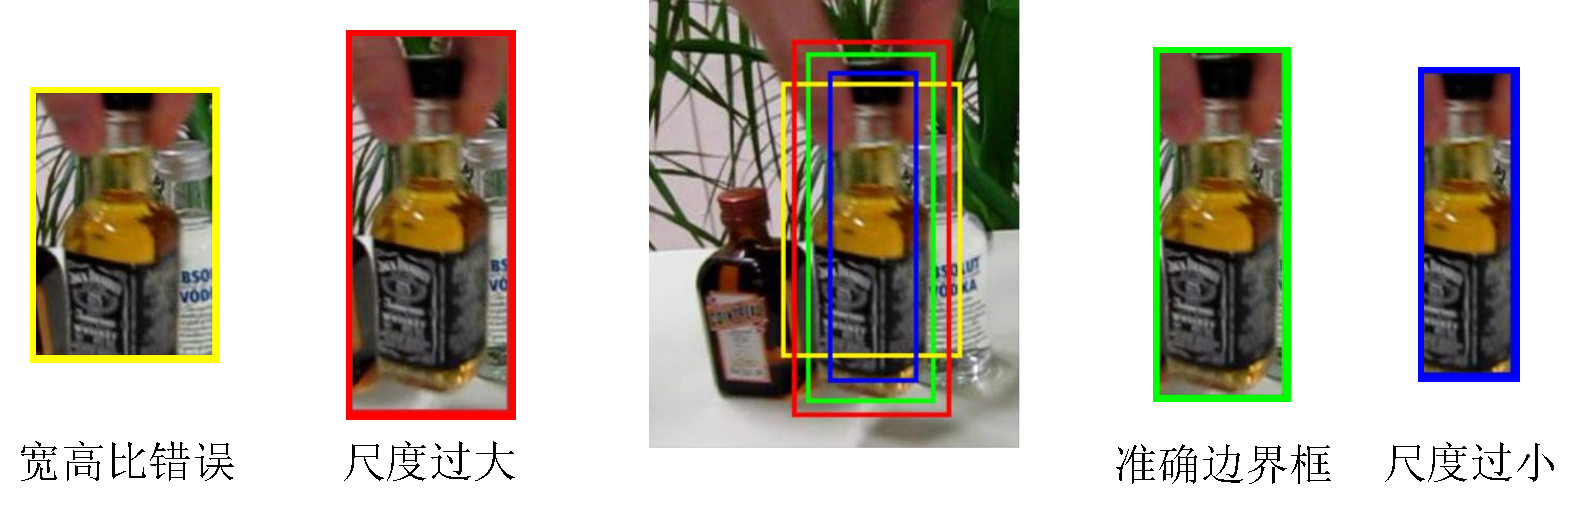
\includegraphics[width=12.5cm]{scaleaspect.pdf}
\caption{尺度和宽高比误差的可视化例子}
\label{scalearerror}
\end{figure}

为了应对视觉跟踪应用中的诸多挑战,跟踪算法正变得越来越复杂。
然而近年提出的基于相关滤波的跟踪器\upcite{mosse,csk,kcf,dsst,act,samf,pbcf} 在取得上佳性能的同时,却十分简单和快速。
这些跟踪器的核心部分都是一个具有分辨能力的滤波器,其输出的卷积结果能够显示出输入图像和跟踪目标的相似度。
由于频率域的点对点操作等价于时间域(图像处理中为空间域)的卷积操作,
上述滤波器能够极其高效地辨识所有循环位移后的输入图像。
但是,滤波器的输入必须是固定大小的图像块,因此基于相关滤波的跟踪器天生缺乏对于目标尺度和宽高比变化的适应力。
尽管一些能够适应尺度变化的变型\upcite{dsst,samf,pbcf}已经出现,但是它们仍局限于预定的尺度采样方式,不够灵活。
此外,在本章已知的范围内,除了\cite{pbcf}以外还没有相关滤波跟踪器能够解决对于目标宽高比的适应性问题。

在目标检测领域,近来具有顶级性能的目标检测系统\upcite{rcnn,spp}均采用了``目标候选''方法来提取可能包含目标物体的候选区域。
该类方法可以在没有任何先验知识的情况下,在输入图像中提取任意尺度、宽高比的候选边界框,如图\ref{detectionproposalres}所示。
目标候选方法不仅能够避免对大量的边界框进行分类,还能预先滤除大部分错误的边界框,大幅提高检测精度\upcite{dpsurvey,dpcompare}。
在本章中,由于具有较高的检测性能和对于跟踪任务的适应性,目标候选生成器EdgeBoxes\upcite{edgeboxes}将被融入跟踪器中,
以提升跟踪器对尺度和宽高比的适应力。

\begin{figure}[htb]
\centering
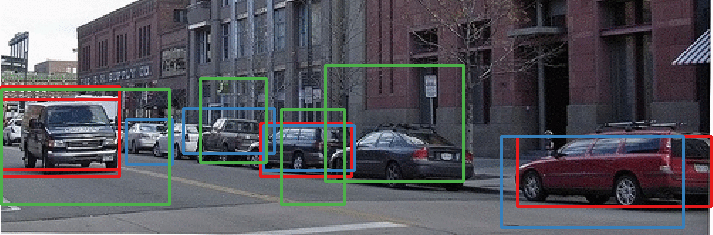
\includegraphics[width=13cm]{detectionproposalres.png}
\caption{生成``目标候选''的可视化例子}
\label{detectionproposalres}
\end{figure}

本章中,KCF\upcite{kcf}这一典型的基于相关滤波的跟踪器将作为跟踪器的主体框架。
通过对输入滤波器的图像特征进行增强,以及采用更为鲁邦的目标模型更新方法,
KCF的辨别力将变得更加鲁邦和准确,足以对灵活的目标候选进行分类。
初步确定目标所在位置后,EdgeBoxes将被用于在其附近生成目标候选。
这些候选边界框经过一个过滤步骤后,将被输入KCF进行再次辨别,以提取出最优的目标候选。
最后,通过一个阻尼更新过程,最优候选边界框将被用于确定最终的目标位置、尺度和宽高比。
本章最终将得到一个集成了目标候选生成器的全新跟踪器,它在公开的大规模测试集中取得了顶级的精度,
并且达到了20.8 FPS(每秒处理的帧数)的跟踪速度。

本章的内容安排如下:第2节介绍与本章紧密相关的现有研究工作;
第3节介绍本章跟踪器框架的基础\pozhehao 核化相关滤波器KCF;
第4节对KCF进行优化,以适应对目标候选的分类任务;
第5节介绍如何将目标候选生成器EdgeBoxes高效地融入跟踪框架中;
第6节将对本章方法进行实验评测和分析;
最后在第7节进行本章的总结。

\section{相关研究}
\subsection{跟踪器的尺度和宽高比适应力}
根据绪论中对跟踪器各模块的功能分析可以看出,运动模型是决定一个跟踪器的尺度和宽高比适应力的关键。
\cite{survey51}基于光流跟踪算法,已被广泛应用于图像对准(Image Registration)。
它通过增量式对齐(Incremental Alignment)来计算两帧中目标物体图像块的仿射变换(Affine Transformation)。
由于仿射变换的参数包含6个自由度,因此该跟踪器可以感知目标物体的位移、尺度变化和旋转。
LSK跟踪器\upcite{lsk}在每一帧中都会预先``猜测''一个目标中心位置并采样候选图像块,
然后使用Mean-Shift聚类方法优化该猜测,以最大化候选图像块和匹配模板的相似度。
由于Mean-Shift优化过程会根据多种尺度反复进行,因此LSK跟踪器能够成功判断当前目标的尺度大小。
上述两个跟踪器中,物体的运动都是通过计算或者优化过程直接得到的,因此其运动模型属于隐式模型。

ASLA\upcite{asla}和SCM\upcite{scm}均采用仿射变换来描述两帧间的目标运动。
与\cite{survey51}根据光流跟踪结果直接计算仿射变换不同,这两个跟踪器将仿射变换的6个参数用6个独立的高斯分布进行建模。
然后,跟踪器将通过不断采样仿射变换参数并进行验证的方式,寻找最为合适的目标位置和尺度。
这种按照概率分布来采样目标状态参数,然后以目标当前状态更新概率分布的方式,属于典型的点滤波(Particle Filtering)运动模型。
VTD\upcite{vtd}跟踪器会同时考虑目标的位置和尺度变化,并用两个高斯分布来分别建模平滑和突发的目标运动。
这两个点滤波运动模型将配合多个不同的观察模型,得出多个跟踪结果,
并通过马尔科夫链蒙特卡洛(Markov Chain Monte Carlo)方法整合出一个最终结果。

此外,还有部分跟踪器使用了特殊方法来获得尺度和宽高比适应力。
为了应对物体非刚性形变带来的大幅度尺度和宽高比变化,HBT\upcite{houghtrack}将图像分割方法加入了跟踪过程。
根据霍夫森林(Hough Forest)得出的反向映射向量将投票决定目标物体的中心位置,
而中心位置将作为前景点输入图割算法Grabcut,以对目标物体和背景进行分割。
由于图像分割得到的是目标物体的细致轮廓,因此HBT可以准确适应目标的尺度和宽高比变化。
但是图像分割计算开销巨大,使得HBT难以用于实时跟踪场景。
TLD\upcite{tld, tldjournal}跟踪算法将Fern随机森林检测器和光流跟踪器进行了整合。
Fern随机森林检测器通过滑动窗口的方式搜索整幅帧图像,找出可能包含目标物体的边界框;
光流跟踪器则根据多个目标特征点的运动,估计目标的整体运动。
这两个模块均能适应目标的尺度和宽高比变化。

\subsection{基于相关滤波的跟踪器}
基于相关滤波的跟踪器通常选择密集采样作为运动模型,即是说,它们通过在图像中密集地采样候选区域并进行辨别,
来检测目标物体的当前位置和状态。
因此,密集采样的模式(例如采样时边界框的大小、形状是否可变)决定了跟踪器对尺度和宽高比的适应力。
MOSSE跟踪器\upcite{mosse}将经过随机仿射变换的目标物体图像作为训练集,用于初始化它的相关滤波器。
但是在跟踪过程中,采样边界框的尺度和宽高比不再变化,滤波器仅用于检测目标的当前位置。
KCF\upcite{kcf}跟踪器是CSK\upcite{csk}的一个扩展版本,它通过利用图像块中的循环模式进行卷积操作,取得了极高的跟踪效率。
KCF还利用``核技巧(Kernel Trick)''来增强了传统的相关滤波器,同时使得滤波器支持多通道的特征。
但是,它仍然没有解决尺度的适应力问题。
作为CSK的另一个固定尺度扩展版本,ACT\upcite{act}采用颜色名(Color Naming)作为特征,并使用了特征压缩方法提高跟踪效率。
此外,ACT还提出了一个更加鲁棒的模型更新策略以提高精度。

SAMF\upcite{samf}在KCF的基础上,通过在采样时加入几种预定义的尺度变化来解决KCF的尺度适应力问题。
相关滤波器将对这些不同尺度的采样样本进行辨别,以找出最佳的目标位置和尺度大小。
不同于SAMF,DSST\upcite{dsst}将两个独立的相关滤波器结合在了一起:一个基于MOSSE,仅用于估计目标位置;
另一个为一维相关滤波器,仅用于确定目标物体尺度。
在每一帧中,DSST首先利用第一个滤波器确定目标位置。
然后在该位置处采样不同尺度的图像块组成``尺度金字塔'',并将其输入第二个滤波器中以估计尺度。
对比SAMF和DSST,可以看出DSST的尺度检测会更加地准确和快速。
因为相关滤波器具有辨别力,可以显式地区分出各个尺度的置信度,并且可以在频率域更快地进行计算。
但是,这两个基于相关滤波的跟踪器都没有针对目标的宽高比变化进行处理。
\cite{pbcf}中提出的跟踪器通过使用多个独立的相关滤波器来同时跟踪目标物体的多个部分,
并将各个滤波器的输出整合为一个响应图。
随后,跟踪器在响应图中按照高斯分布采样不同的位置、尺度和宽高比,并使用一个贝叶斯框架对采样样本进行评价,
以确定目标物体的当前状态。
显然,上述跟踪器均依赖于预先定义好的采样模式,因而灵活性严重受限,无法处理突发、快速的尺度和宽高比变化。

STC\upcite{stc}是一个例外,它在估计目标尺度时使用的运动模型为隐式模型。
严格来讲,STC并不是基于相关滤波的,但是其推导出的核心算法与相关滤波器十分类似。
它对目标和目标周围区域的上下文时空关系进行了重新建模,并将尺度的变化显式地体现在了模型中。
因此尺度变化可以被直接计算出来而无需通过采样,但是宽高比的变化仍然无法被感知。

\section{使用核化相关滤波器进行视觉跟踪}
作为本章跟踪器的主体框架和基础,核化相关滤波器KCF的主要目标是训练一个线性模型:
\begin{equation}
f(\mathbf{z})=\left\langle\mathbf{w}, \mathbf{z}\right\rangle ,
\label{kcfeq1}
\end{equation}
其中函数值$f(\mathbf{z})$显示了输入图像块$\mathbf{z}$与目标物体的相似程度,即线性模型的响应值。
$\left\langle\cdot, \cdot\right\rangle$代表内积,
$\mathbf{w}$为该线性模型的参数矩阵。
公式\ref{kcfeq1}即是KCF的观察模型,即判断候选图像块是否包含目标物体的模块。
KCF将上一帧的目标物体边界框进行放大,得到一个上下文窗口,然后根据该窗口提取图像块。
该图像块的每一次循环位移都将产生一个候选图像块$\mathbf{z}$,并将被输入观察模型,以计算其中包含目标的概率。
显然,若当前帧中目标物体在上下文窗口内,那么目标物体一定位于某一个循环位移后的图像块的中心,
该图像块的$f(\mathbf{z})$也应当具有最大值。
可视化的例子如图\ref{kcf1}所示。显然,循环位移就是KCF的运动模型。
由于会对所有循环位移进行辨别,因此它还是一种密集采样运动模型。

\begin{figure}[htb]
\centering
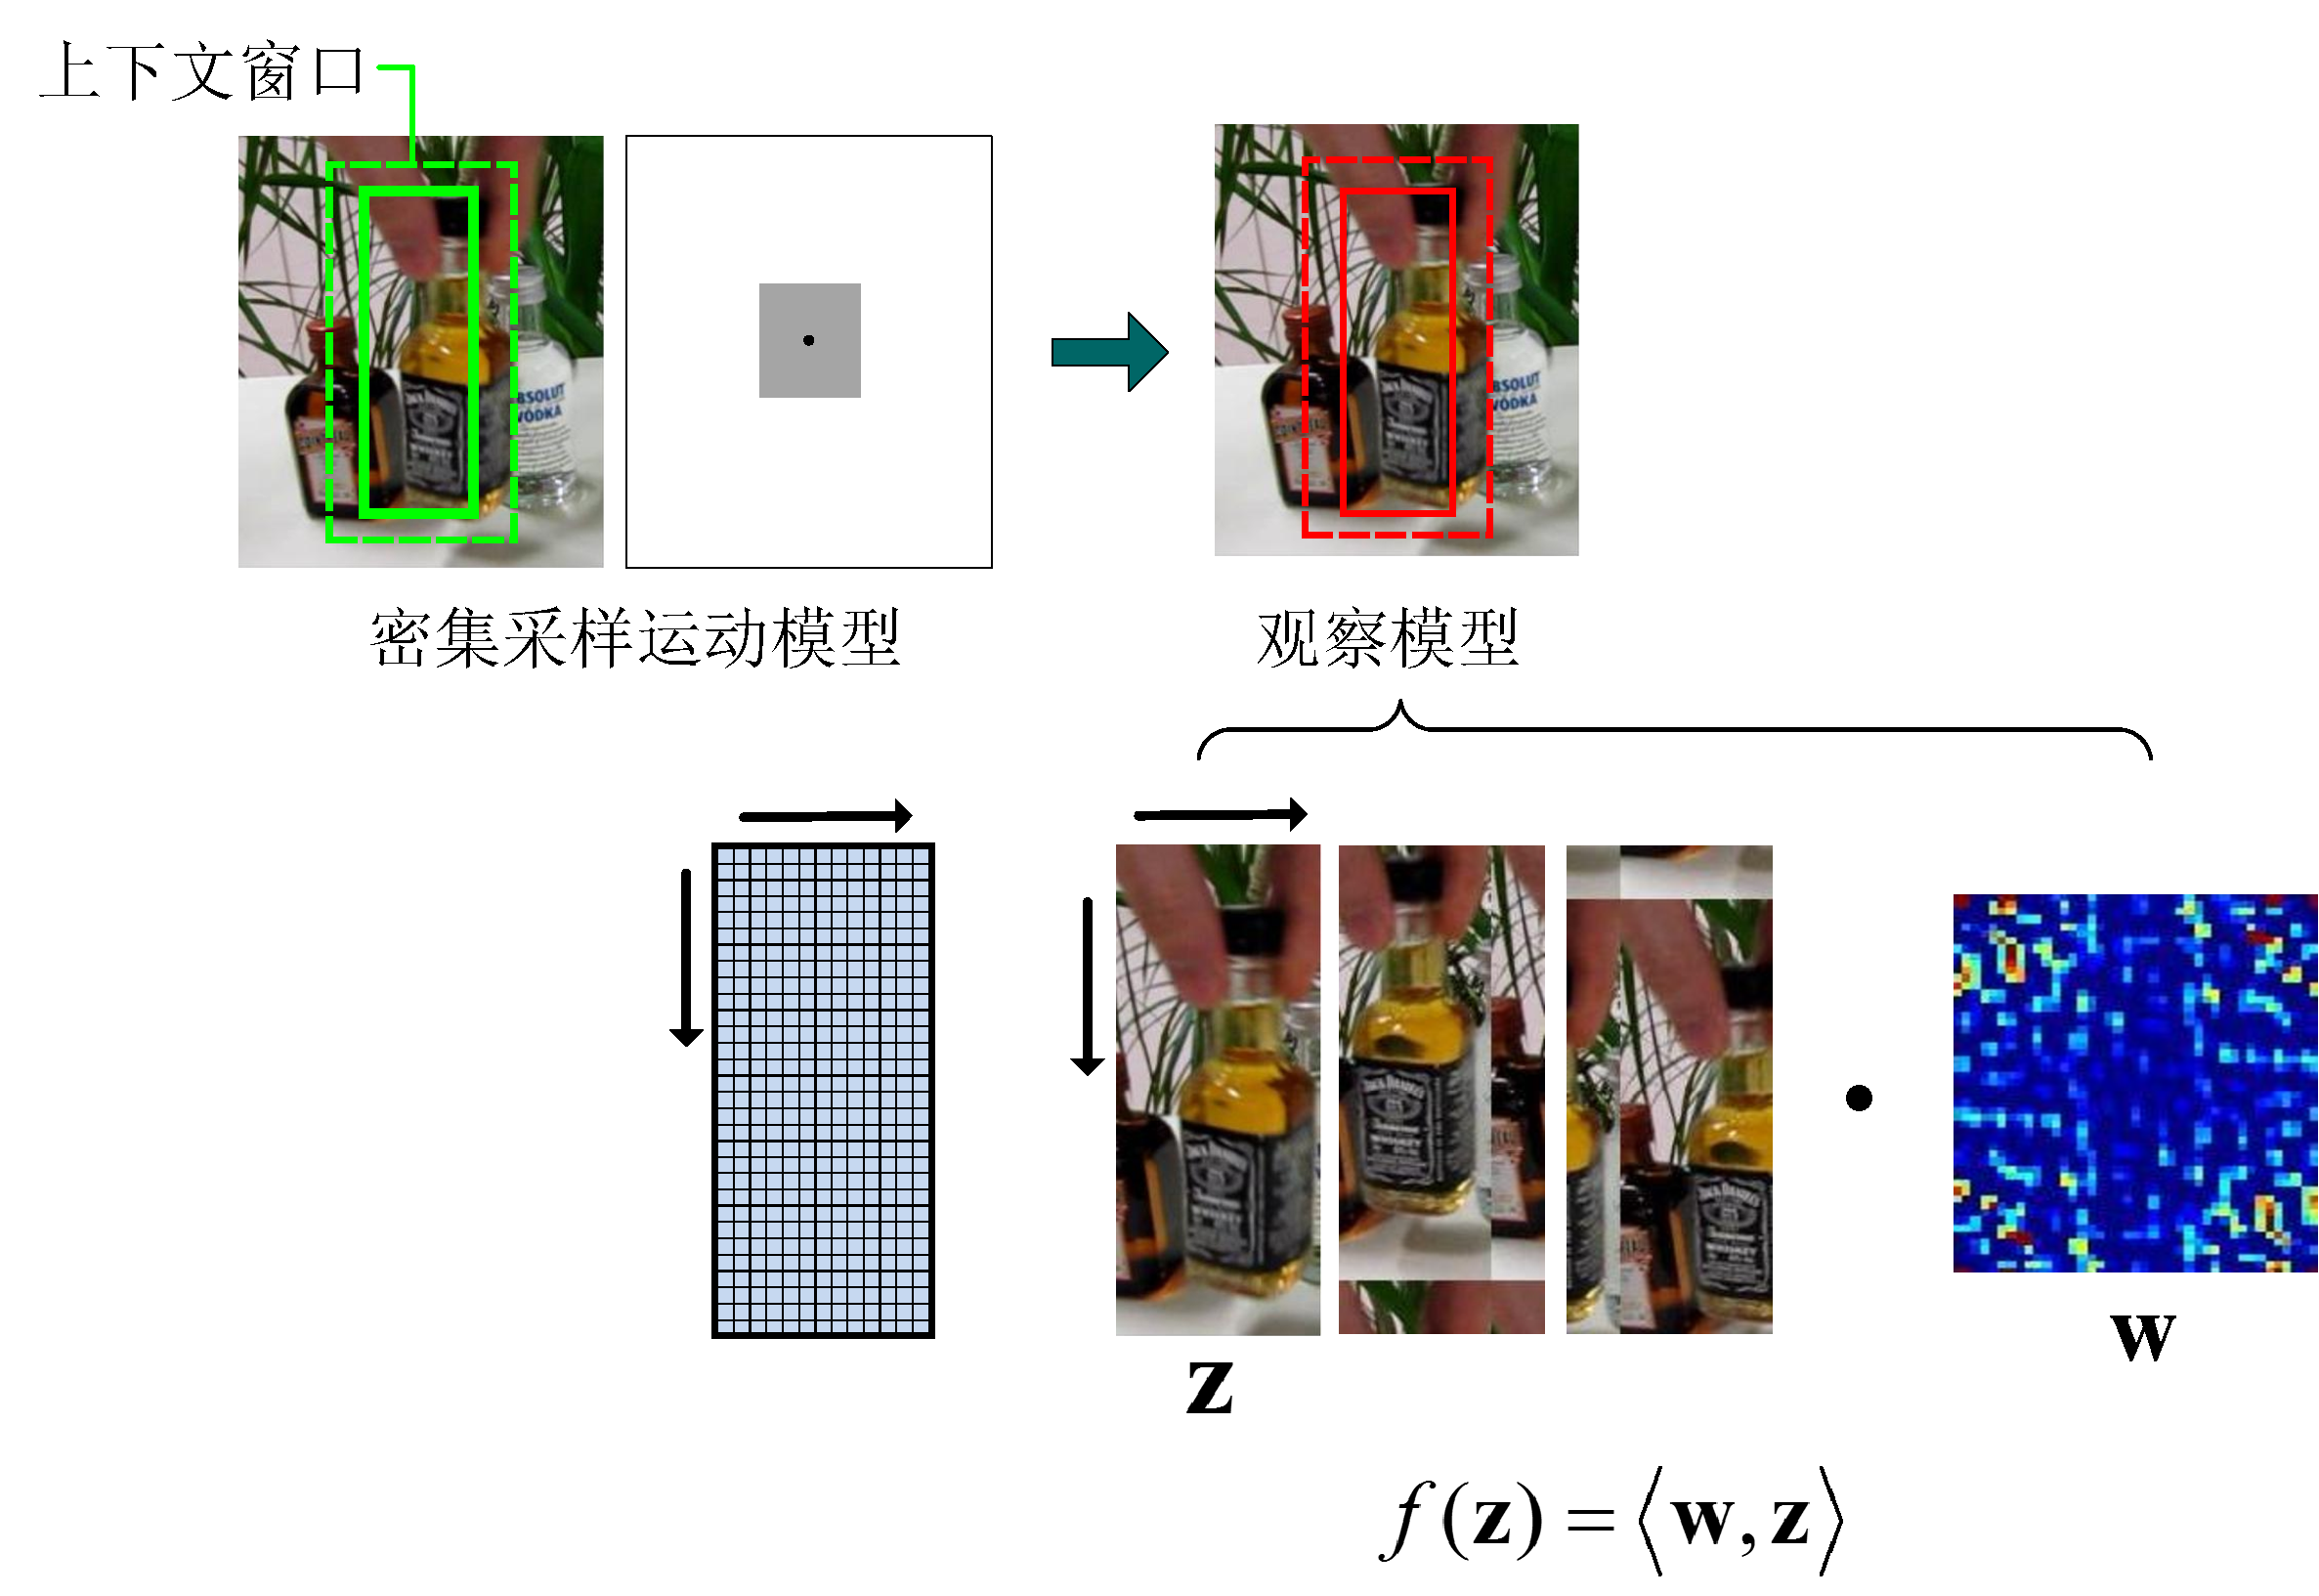
\includegraphics[width=11cm]{kcf1.pdf}
\caption{KCF的运动模型和观察模型}
\label{kcf1}
\end{figure}

求解参数矩阵$\mathbf{w}$的过程,就是求解``岭回归(Ridge Regression)''问题的过程。该求解或者说训练的目标函数为:
\begin{equation}
	\underset{\mathbf{w}}{\min}\,\sum_{m,n}\left(f(\mathbf{x}_{m,n})-y_{m,n}\right)^{2}+\lambda\left\Vert \mathbf{w}\right\Vert ^{2}.
	\label{rrmin}
\end{equation}
$\mathbf{x}_{m,n}$是用于训练的图像块,$\lambda$被称作规则化参数(Regularization Parameter),用于防止过拟合。
$y_{m,n}$是回归目标,即对于输入的$\mathbf{x}_{m,n}$所期望的$f(\mathbf{x}_{m,n})$值。
在KCF中,$\mathbf{x}$代表目标物体图像块,即一个``真值''。
$\mathbf{x}_{m,n}$是由$\mathbf{x}$纵向循环位移$m-1$个像素,再横向循环位移$n-1$个像素所得到的图像块。
显然$\mathbf{x}_{1,1}=\mathbf{x}$,因此其对应的$y_{1,1}$应当具有最大值,即$y_{1,1}=1$。
若将所有的$y_{m,n}$组成一个矩阵$\mathbf{y}$,那么理想情况下,$\mathbf{y}$应当符合一个将峰值循环位移到左上角的二维高斯函数。

KCF通过使用高斯核函数,将公式\ref{kcfeq1}变换到了对偶空间(Dual Space):
\begin{equation}
\begin{aligned}
	f(\mathbf{z})=\left\langle\mathbf{w}, \mathbf{z}\right\rangle&=\sum_{m,n}\alpha_{m,n}\left\langle\mathbf{z},\mathbf{x}_{m,n}\right\rangle=\sum_{m,n}\alpha_{m,n}\ g\negthinspace\left(\mathbf{z},\mathbf{x}_{m,n}\right),\label{kcf-kernelmodel}
\end{aligned}
\end{equation}
其中$g\negthinspace\left(\cdot, \cdot\right)$代表高斯核函数,它取代了原式中的内积计算。
相对应的,KCF的运动模型和观察模型也变为图\ref{kcf2}所示。
计算$f(\mathbf{z})$值的过程,实际上变为了将候选图像块$\mathbf{z}$(图中标记为\textbf{C})和每一个训练图像块$\mathbf{x}_{m,n}$进行对比的过程,
参数矩阵$\mathbf{w}$也被新参数$\alpha_{m,n}$所组成的矩阵$\boldsymbol{\alpha}$所替代。
而训练图像块集合中,循环位移较小的必然与原目标物体图像块相似,成为了正样本(图中标记为\textbf{P});循环位移较大的则成为了负样本(图中标记为\textbf{N})。

\begin{figure}[htb]
\centering
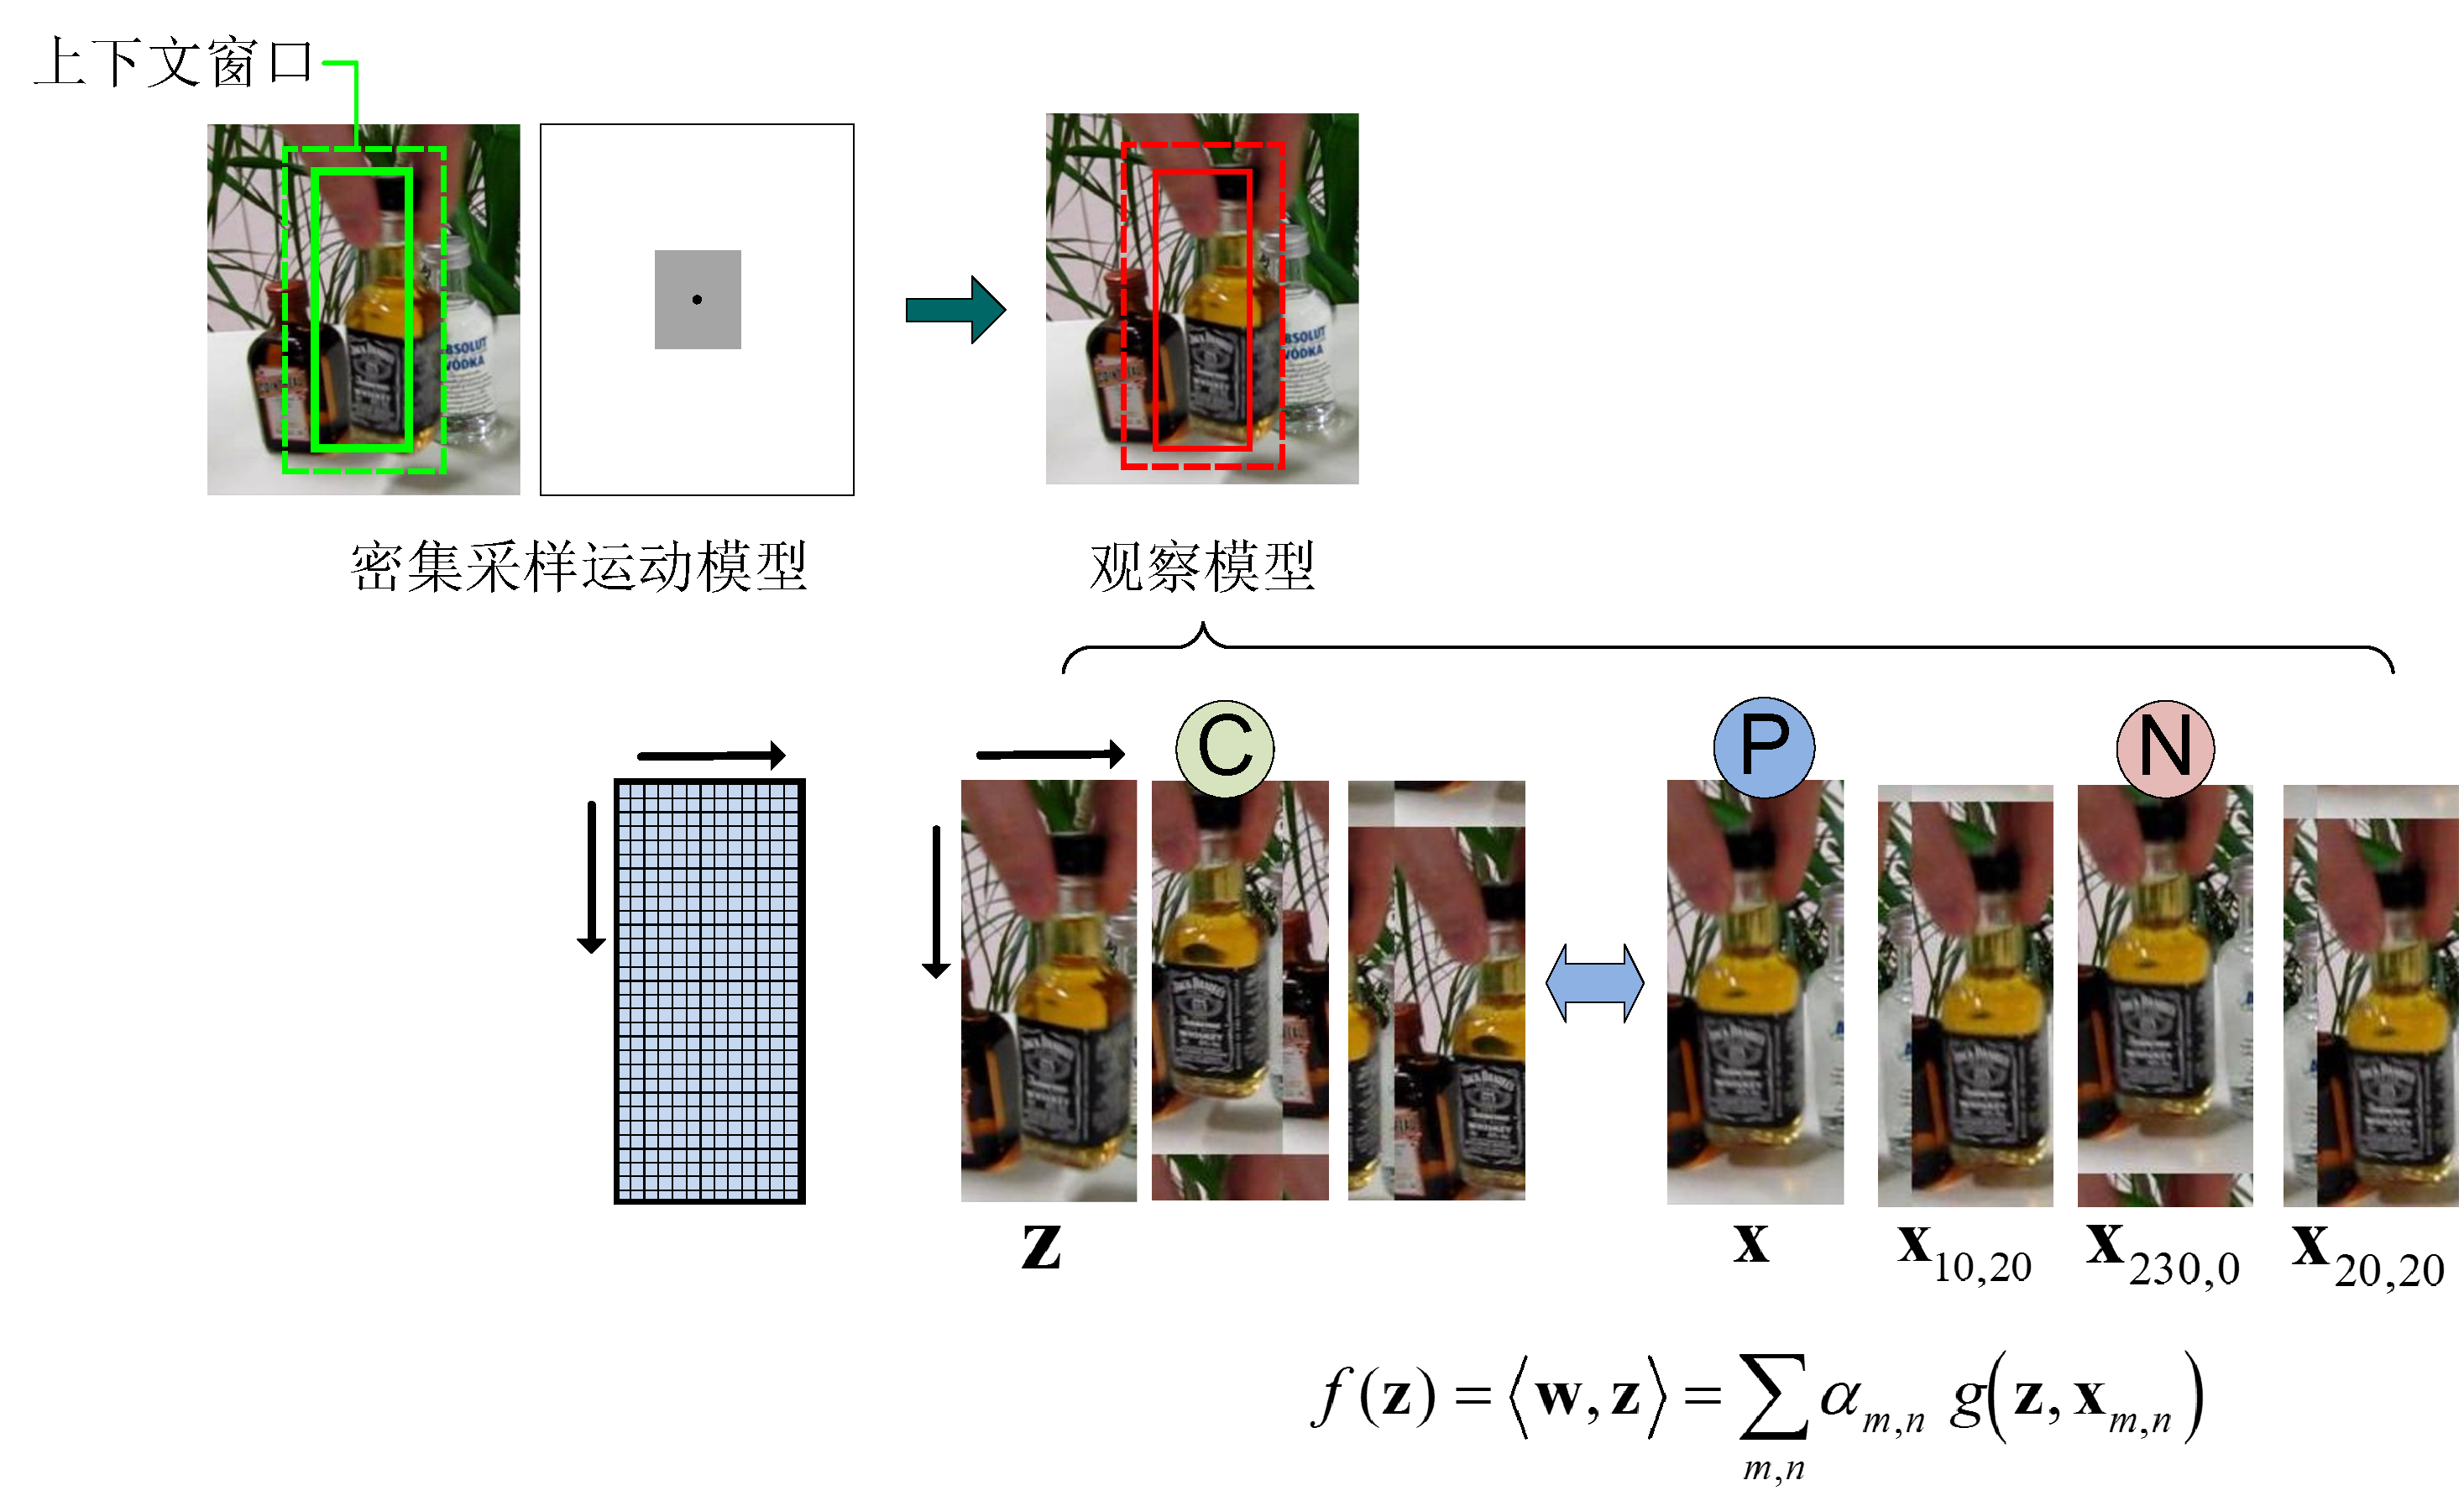
\includegraphics[width=13cm]{kcf2.pdf}
\caption{使用高斯核后的KCF运动模型和观察模型}
\label{kcf2}
\end{figure}

通过利用各个$\mathbf{x}_{m,n}$间的循环关系,以及卷积定理(Convolution Theorem),公式\ref{rrmin}的解为:
\begin{equation}
	\hat{\boldsymbol{\alpha}}=\frac{\hat{\mathbf{y}}}{\hat{\mathbf{k}}{}^{\mathbf{x}_{1,1}\mathbf{x}_{1,1}}+\lambda}.\label{kcf_learning}
\end{equation}
上式中的$\hat{\cdot}$代表离散傅里叶变换(DFT),$\mathbf{k}$ 代表核化相关算子,其定义为:
\begin{equation}
\begin{aligned}
%	\mathbf{k}^{\mathbf{x' x''}}=\exp\left(-\frac{1}{\sigma^{2}}\left(\left\Vert \mathbf{x'}\right\Vert ^{2}+\left\Vert \mathbf{x''}\right\Vert ^{2}-2\mathcal{F}^{-1}\left(\sum_{c}\,\hat{\mathbf{x'}}_{c}^{*}\cdot\hat{\mathbf{x''}}{}_{c}\right)\right)\right), \label{kcf-kr}
	&\mathbf{k}^{\mathbf{x' x''}}=
	&\exp\left(-\frac{1}{\sigma^{2}}\left(\left\Vert \mathbf{x'}\right\Vert ^{2}+\left\Vert \mathbf{x''}\right\Vert ^{2}
	-2\mathcal{F}^{-1}\left(\sum_{c}\,\hat{\mathbf{x'}}_{c}^{*}\cdot\hat{\mathbf{x''}}{}_{c}\right)\right)\right), \label{kcf-kr}
\end{aligned}
\end{equation}
式中$\sigma$是高斯核函数的带宽,$\mathcal{F}^{-1}$代表离散傅里叶逆变换,${*}$代表复共轭算子,
下标$c$代表图像特征向量的第$c$个通道, $\exp$即指数函数。
公式\ref{kcf-kr}中的所有运算操作,包括$\exp$,都是逐元素进行的。
公式\ref{kcf_learning}将负责训练相关滤波器,即在第一帧中用用户标注出的或者检测到的目标物体图像块初始化相关滤波器。

同样利用循环关系和卷积定理,KCF可以同时计算出输入图像块$\mathbf{z}$的所有循环位移所对应的响应值。
也就是说,公式\ref{kcf-kernelmodel}可变换为:
\begin{equation}
	\hat{\mathbf{f}}(\mathbf{z})=\hat{\mathbf{k}}^{\overline{\mathbf{x}}\mathbf{z}}\cdot\hat{\boldsymbol{\alpha}},\label{kcf-detection}
\end{equation}
其中$\overline{\mathbf{x}}$被称作当前目标外观。
由于目标物体外观在跟踪中会不断变化,因此公式\ref{kcf-kernelmodel}中的$\mathbf{x}$也会不断更新,并记为$\overline{\mathbf{x}}$。
$\mathbf{z}$的所有循环位移的响应值$f$组成了矩阵$\mathbf{f}$,
且各个响应值在$\mathbf{f}$中的位置,与循环位移的像素数目相对应,即$\mathbf{f}[m,n]=f(\mathbf{z}_{m,n})$。
因此,根据$\mathbf{f}$中最大元素所在的位置,可以找出最接近当前目标外观的$\mathbf{z}_{m,n}$,
从而直接推断出目标物体中心在上下文窗口中的位置。
公式\ref{kcf-detection}是KCF的核心,将负责在每一帧中检测目标物体的中心位置。
而它又是由参数矩阵$\boldsymbol{\alpha}$和当前目标外观$\overline{\mathbf{x}}$所共同决定的,
因此这两个矩阵也被称作``KCF的模型''。

每当在新的一帧中跟踪到目标物体后,KCF都会更新自己的模型,以适应光照变化、目标旋转、形变等导致的目标外观变化。
KCF的模型更新策略非常简单直接,就是进行线性插值。
记当前帧中目标物体图像块为$\mathbf{x}_i$,对于参数矩阵,首先重新训练一个参数矩阵$\boldsymbol{\alpha}_i$,然后进行线性插值:
\begin{equation}
	\hat{\boldsymbol{\alpha}_i}=\frac{\hat{\mathbf{y}}}{\hat{\mathbf{k}}{}^{\mathbf{x}_i\mathbf{x}_i}+\lambda}, \\ \ \ \ 
	\boldsymbol{\alpha}=\eta{\boldsymbol{\alpha}_i} + ( 1-\eta )\boldsymbol{\alpha}.
	\label{kcf_learning2}
\end{equation}
对于目标外观,则直接进行线性插值:
\begin{equation}
\overline{\mathbf{x}}=\eta\mathbf{x}_i+(1-\eta)\overline{\mathbf{x}}.
\end{equation}


\section{图像特征整合和鲁棒更新}
在跟踪过程中加入目标候选生成器后,相关滤波器需要辨别的不仅是循环位移后的图像块,
还包括各种尺度大小和宽高比的目标候选。
由于候选图像块的灵活性和数量增加,各种干扰因素也将增加,对相关滤波器的精度和鲁棒性也提出了更高的要求。

为了提升精度,本节将首先加强KCF的目标描述。
KCF所使用的``梯度直方图(HOG)''特征被扩展为HOG、亮度和颜色名三者结合的混合特征。
这种特征整合的方法在SAMF\upcite{samf}和ACT\upcite{act}中均有使用,但是本节不对特征进行压缩。
这三种特征的简要介绍如下:
\begin{compactitem}
\item{\textbf{亮度}:要计算亮度,需要先将彩色图像转换为灰度图像。假设图像块按RGB三个通道存储,则一个像素的灰度可计算为:
$0.2989 * R + 0.5870 * G + 0.1140 * B$。随后,将每个像素的灰度值减去整个图像块的平均灰度值,即得到了各个像素的亮度值。}
\item{\textbf{梯度直方图}\upcite{hog}:在亮度图的基础上,首先对于每一个像素点,计算其横向和纵向的亮度梯度。
然后根据横、纵亮度梯度,计算出每个像素的梯度方向。之后将图像分为$4\times4$细胞单元(Cell)组成的网格,
并在每一个细胞单元中对9个离散的梯度方向进行投票。每个像素点的投票均具有权值,且该权值就是梯度的大小。
最后将多个细胞单元组合成较大的区块,并对这些区块中的梯度方向投票进行统计,得出梯度直方图特征。}
\item{\textbf{颜色名}\upcite{colornaming}:之所以将这种特征命名为颜色名,是因为它将所有的颜色按照语言学分为了11类,
即11类人类常用的颜色名字。这样的颜色分类更接近于人类的感知,且已经在物体检测\upcite{colornaminguse2}和动作识别\upcite{colornaminguse1}领域取得了很好的效果。这里直接利用\cite{colornaming}中的方法将RGB 3个通道的值向11个颜色名通道进行映射,
得到颜色名特征。}
\end{compactitem}
将这三种特征同时用于目标描述的原因是它们之间有很好的互补性:
亮度,顾名思义,描述的是各个像素的明亮程度,但是缺乏对不同颜色的区分度;
梯度直方图更着重于描述图像中的轮廓和形状,但是难以区分亮度和颜色;
颜色名是当前分类器常用的颜色特征,有着明显优于传统RGB颜色表达的性能。


To improve precision, we extend the HOG feature used in original KCF to a combination of HOG, intensity, and color naming,
similarly to SAMF~\citep{samf} and ACT~\citep{act} but without feature compression.
By simply concatenating the three features, the target appearance with feature integration shown in Fig.~\ref{process}(g) now has 42 channels, and can be used in training and detection
according to Eq.~(\ref{kcf-kr}).

The utilization of simple linear interpolation as model updating scheme in KCF is proved to be suboptimal~\citep{act},
because only the current frame is taken into account while updating the model, and the contribution of previous frames in model
fades out too fast exponentially.
To make KCF more robust, our tracker adopts the robust model updating scheme presented in ACT instead (shown as the bottom arrow in Fig.~\ref{process}),
which considers the target patches in current frame and all previous frames simultaneously. 
Note that although previous target patches are explicitly considered, they are implicitly encoded into the scheme, so that
the derived updating formula only requires the current target patch as follows.
In each new frame indexed by $i$, after a patch $\mathbf{x}_i$ containing the target is detected, % using equation \ref{kcf-detection}, 
the numerator and denominator of 
the coefficient matrix $\hat{\boldsymbol{\alpha}}$ are updated
separately to reproduce a new one:
\begin{equation}
\begin{aligned}
	&\hat{\boldsymbol{\alpha}_N}=\eta\hat{\mathbf{k}}^{\mathbf{x}_i \mathbf{x}_i} \cdot \hat{\mathbf{y}} + (1-\eta){\hat{\boldsymbol{\alpha}_N}};
	\\
	&\hat{\boldsymbol{\alpha}_D}=\eta\hat{\mathbf{k}}^{\mathbf{x}_i \mathbf{x}_i} \cdot (\hat{\mathbf{k}}^{\mathbf{x}_i \mathbf{x}_i} +
	\lambda) + (1-\eta){\hat{\boldsymbol{\alpha}_D}}.\label{kcfdp-updating}
\end{aligned}
\end{equation}
Here $\hat{\boldsymbol{\alpha}}={{\hat{\boldsymbol{\alpha}_N}}}/{{\hat{\boldsymbol{\alpha}_D}}}$, and $\eta$ is the learning rate.
The target appearance $\overline{\mathbf{x}}$ is still updated by linear interpolation: $\overline{\mathbf{x}}=\eta\mathbf{x}_i+(1-\eta)\overline{\mathbf{x}}$.
For detailed rationales and derivations, please refer to \cite{act}.


\section{将``目标候选''嵌入跟踪器中}
bmvc论文

\section{实验结果与分析}
\subsection{实验设置}
\subsubsection{参数设置}
\subsubsection{测试集和对照组构成}
介绍OTB50,介绍自己提取的子集
\subsubsection{评价标准}
介绍CLE和IoU,介绍精确度图和成功率图
\subsection{尺度和宽高比适应力评测}
\subsection{整体性能评测}

\section{小结}
